\section{Personagens}

\subsection{Introdução}
O jogo apresentará duas classes de dificuldades ao personagem principal 
(ou jogador): de percurso e de inimigos. As dificuldades de percurso serão 
aquelas apresentadas pelo ambiente e que exigirá a habilidade de locomoção 
do personagem, tal como salto ou desvio de obstáculos. As dificuldades 
de inimigos serão aquelas que exigirão a habilidade de ataque e defesa 
do personagem quando em confronto com um inimigo.

Nas seções a seguir são apresentadas as formas de controle dos estados 
do personagem principal, os inimigos e suas respectivas características 
e, por fim, o cenário e seus desafios.

\subsection{Estados do Personagem Principal}
Na primeira fase do jogo, haverá duas barras para que o jogador possa 
controlar os estados do per-sonagem principal, ou seja, a condição física 
dele: a barra de vida e a barra de energia.
 
\subsubsection{Barra de Vida}
A barra de vida exibe o nível de vitalidade do personagem principal. 
A Figura 1 apresenta um esboço desta barra, que começa completa, com
100 pontos percentuais. São dois os fatores que influenciarão no 
decaimento do nível: ataques sofridos e barra de energia vazia. Os ataques 
sofridos condizem com os ata-ques dos animais que o personagem encontrará
nos cenários da primeira fase. O valor que será decremen-tado da barra de 
vida dependerá da força de ataque do animal em específico. Sobre a barra de 
energia vazia e a forma de recuperação da força vital do personagem, estas
são tratadas na subseção a seguir.

\begin{figure}[H]
 \centering
 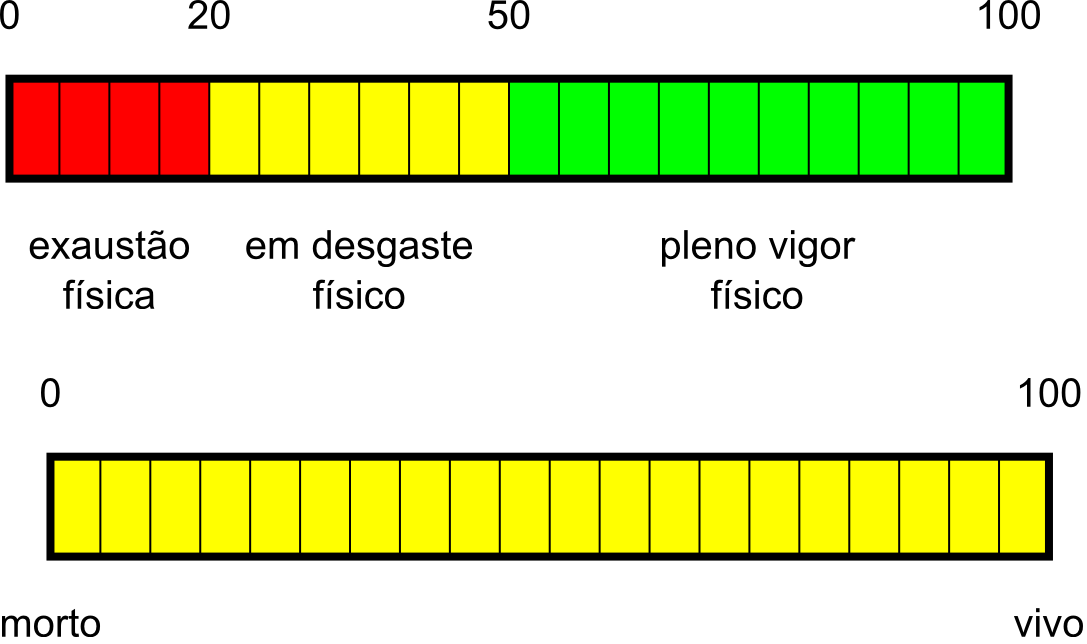
\includegraphics[scale=3]{BarraDeEnergia.png}
 \caption{Esboço das barras de vida (acima) e energia (abaixo).}
 \label{img:energia}
\end{figure}

\subsubsection{Barra de Energia}
A barra de energia exibe o nível de resistência física do personagem principal, 
ou seja, a capacidade dele para desenvolver um esforço físico. A Figura 1 apresenta 
um esboço desta barra, que inicia cheia. No intervalo de 50 a 100, destacado em 
verde, o personagem estará em pleno vigor físico. Ele conseguirá correr e pular 
alto ou longas distâncias. No intervalo de 20 a 50, destacado em amarelo, o 
personagem começará a sofrer um desgaste físico. Ele passará a correr cada vez 
mais lento e a saltar alturas e distâncias cada vez menores até chegar à exaustão 
física – a função para controle da capacidade de esforço físico do persona-gem é 
apresentada no Gráfico 1. No intervalo de 0 a 20, o personagem já não conseguirá 
mais correr e nem pular, apenas andar.

\begin{figure}[H]
 \centering
 \includegraphics[scale=2.5]{VelocidadeDeDeslocamentoEPulo.png}
 \caption{Relação entre a capacidade de esforço físico e a energia
do personagem.}
 \label{img:velocidade}
\end{figure}

Os fatores que influenciarão no decaimento do nível de resistência física 
do personagem são: deslocamento, pulo e golpe. No deslocamento, o nível de 
energia deverá reduzir linearmente em função da distância percorrida pelo 
personagem. A cada pulo ou golpe realizado pelo personagem será decrementado 
ao nível de energia 1 e 1/2 ponto percentual, respectivamente. Se a barra de 
energia estiver vazia, estes fatores deverão interferir, na mesma proporção, 
no nível de vitalidade do personagem. Para elevar ambos os níveis de 
resistência física e de vitalidade, o personagem deverá matar e, em 
seguida, se alimentar dos animais que ele encontrará pelo caminho. Cada 
animal tem o seu valor energético específico.

\subsection{Personagens}
Na primeira fase, os inimigos do personagem principal serão os animais da floresta. 
Haverá cinco espécies de animais: cobra, urso, abelha, jacaré e tigre. Cada espécie 
terá suas características específicas. Estas são apresentadas na Tabela 1, em que K 
é um valor constante e p.p. é a abreviação de pontos percentuais.

\begin{figure}[H]
 \centering
 \includegraphics[scale=1]{tabela.png}
 \caption{}
 \label{img:tabela}
\end{figure}

\subsection{Personagem principal}
\subsubsection{Descrição física e psicológica}
Medrash é o personagem principal, o qual será controlado pelo jogador. Ele
 possui cerca de 20 anos de idade, 1,65 m de altura e 70 Kg. Com um corpo
 magro, mas com músculos definidos, é muito forte, sendo tipicamente um
 caçador.

Ele é um caçador da tribo Ari e marido de Sora. Medrash tem sua esposa e
 amigos sequestrados no inicio do jogo e seu objetivo principal é 
resgatalos.

Medrash enfrenta diferentes inimigos ao longo do jogo. É corajoso,
 determinado e não desiste de resgatar seus companheiros mesmo diante de
 todos os perigos enfrentados ao longo do caminho. É um homem bom e astuto,
 oferecendo ajuda a uma tribo aliada e juntando forças com os mesmos a fim
 de enfrentar a poderosa tribo Luskan.

\subsubsection{Concepção artística}
O Modelo base de Medrash está mostrado na figura \ref{img:medrash}

\begin{figure}[H]
 \centering
 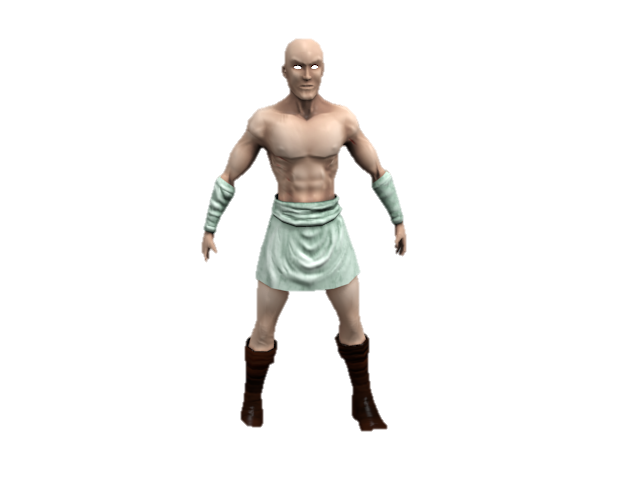
\includegraphics[scale=1]{Imagens/medrash01.png}
 \caption{Medrash.(Fonte:Htp://www.blendswap.com/blends/characters/shaolin/)}
\label{img:medrash}
\end{figure}

\subsubsection{Armas do personagem principal}
\begin{itemize}
\item {\bf Porrete}
O porrete é a arma inicial de Medrash. Simples, rápida e fácil de usar,
 esta arma pode ser utilizada para atacar a maior parte dos inimigos da
 primeira fase.

A Figura \ref{img:porrete} mostra uma concepção artística desta arma.

\begin{figure}[H]
 \centering
 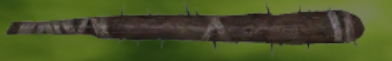
\includegraphics[scale=1]{Imagens/porrete01.png}
 \caption{Exemplo de porrete. (Fonte:Jogo Infinity Blade.)}
\label{img:porrete}
\end{figure}

\item {\bf Lança}
A lança é a segunda arma de Medrash, encontrada ainda na primeira fase,
 podendo ser adquirida de um guerreiro morto. Ela apresenta um grande poder
 de perfuração, sendo assim, mais eficiente que o porrete para caçar
 tigres.

A concepção artistica da lança está na figura \ref{img:lanca}.

\begin{figure}[H]
 \centering
 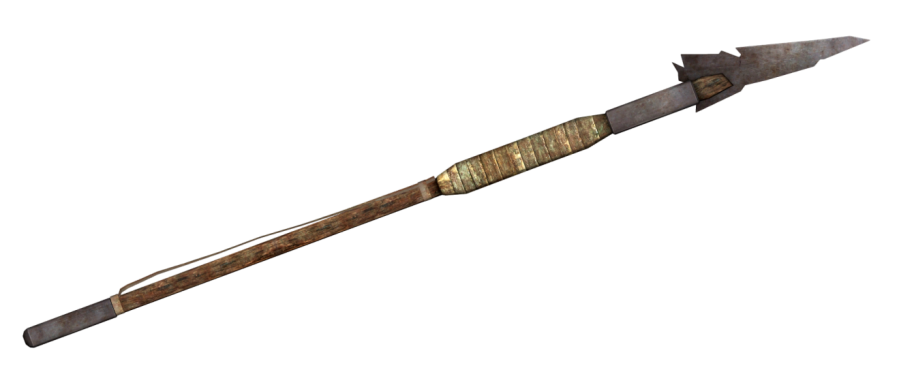
\includegraphics[scale=0.6]{Imagens/lanca01.png}
 \caption{Exemplo de lança. (Fonte: Htp://images.wikia.com/fallout/images/e/e7/SpearFNV.png)}
\label{img:lanca}
\end{figure}


\item {\bf Machado}
Adquirido na segunda parte da fase 2, é uma das melhores armas de Medrash
 para lutar contra a furiosa tribo Luskan. (Detalhar mais sobre a arma).

O conceito artístico do machado pode ser encontrado na figura 
\ref{img:machado}.

\begin{figure}[H]
 \centering
 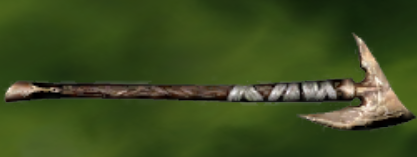
\includegraphics[scale=1]{Imagens/machado01.png}
 \caption{Exemplo de machado. (Fonte: Jogo Infinity Blade)}
\label{img:machado}
\end{figure}

\end{itemize}

\subsection{Personagens Secundários}
\subsubsection{Sora}
Sora é mulher de Medrash, vivendo pacificamente na tribo Ari. Sequestrada
 por Balazar para ser escravizada, precisa da ajuda de Medrash para poder
 ser livre novamente.
\begin{itemize}
\item {\bf Descrição física}
Com aproximadamente 18 anos, com 1.55 m de altura e 50 Kg, 
\item {\bf Concepção artística}
O modelo de Sora está demonstrado na figura \ref{img:sora}.

\begin{figure}[H]
 \centering
 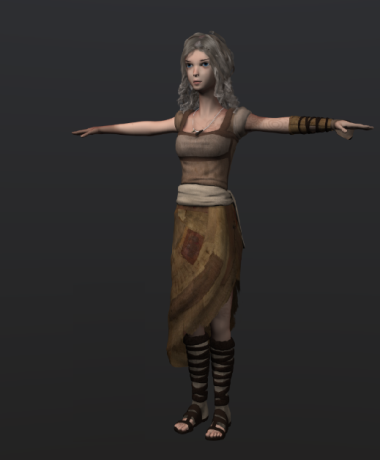
\includegraphics[scale=0.8]{Imagens/sora01.png}
 \caption{Sora.(Fonte:Htp://www.blendswap.com/blends/characters/womanc/)}
\label{img:sora}
\end{figure}


As animações para este personagem são:
\begin{itemize}
\item Ficar parada (gritando, movimentando-se);
\item Corre.
\end{itemize}
\end{itemize}

\subsubsection{Gardain}
Um dos principais guerreiros da tribo Ari, a tribo de Medrash, e o único
 sobrevivente do ataque da tribo Luskan. Ao retornar de sua caçada, Medrash
 vê sua tribo totalmente devastada, restando apenas Gardain como
 sobrevivente. Mesmo estando muito machucado, Gardain conta a Medrash que
 os Luskans fizeram todos da tribo prisioneiros, inclusive sua amada Sora. 
\begin{itemize}
\item {\bf Descrição Física}
Gardain é um guerreiro forte, porém, devido a batalha com a tribo Luskan
 encontra-se esgotado e com diversos ferimentos pelo corpo.
\item {\bf Concepção Artística}
O modelo que servirá como base para a criação de Gardain é apresentado na
 Figura \ref{img:gardain}. Alterações de vestimenta e maiores detalhes
 serão acrescentados para a concepção do personagem.

\begin{figure}[H]
 \centering
 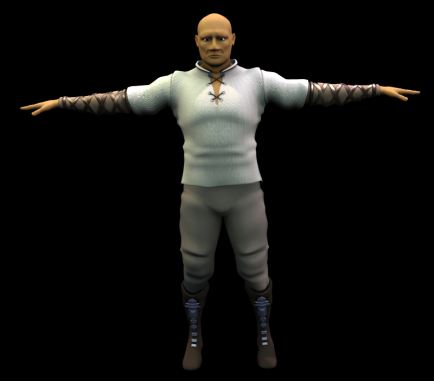
\includegraphics[scale=1]{Imagens/gardain01.png}
 \caption{Modelo para a criação de Gardain(Fonte: Htp://www.blendswap.com/blends/characters/)}
\label{img:gardain}
\end{figure}


\end{itemize}
\subsubsection{Rangrim}
Rangrim é o líder da tribo dos Mara-kai. Ao chegar na tribo, Medrash
 encontra-o ferido após ataque da tribo Luskan. Rangrim informa Medrash de
 que os Luskan pretendem atacar a tribo aliada Akanul, a maior e mais
 importante da região. Experiente e sábio, Rangrim conhece bem os caminhos
 e perigos da região, e indica a Medrash um atalho através das montanhas
 Kabalus, o que permitirá que Medrash chegue a tribo Akanul muito antes dos
 Luskans.
\begin{itemize}
\item {\bf Descrição Física}
Ancião, Rangrim é magro e de baixa estatura. Cabelos e barba branca,
 Rangrim anda de maneira curvada devido a idade avançada.
\item {\bf Concepção Artística}
O ancião apresentado na Figura \ref{img:rangrim} será utilizado para a criação
 do personagem Rangrim. Alterações de vestimenta serão realizadas para que
 se adeque ao período do jogo.

\end{itemize}
\begin{figure}[H]
 \centering
 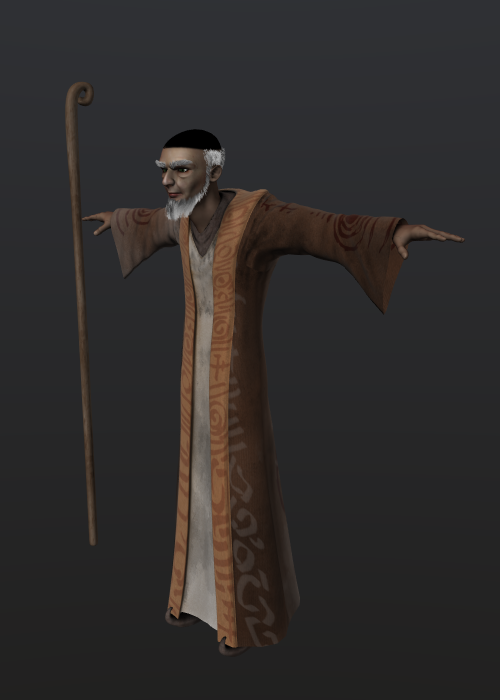
\includegraphics[scale=0.5]{Imagens/rangrim01.png}
 \caption{Modelo de ancião para a criação do personagem Rangrim. (fonte: Htp://www.blendswap.com/blends/characters/religious man/)}
\label{img:rangrim}
\end{figure}

\subsection{Inimigos}
\subsubsection{Cobra}
Não é um inimigo direito de Medrash, só ataca quando se sente ameaçada. A
 cobra é a segunda menor criatura do jogo atrás apenas da abelha. Ela
 patrulha uma determinada área rastejando e, caso o personagem principal se
 aproxime, esta fica enrolada em posição de ataque efetuando bote em forma
 de mordida caso a distância diminua. Se o personagem principal se
 distanciar a cobra volta a patrulhar a área. A cobra está presente apenas
 na primeira fase do jogo.
\begin{itemize}
\item {\bf Descrição Física}
Como mencionado, a cobra é um dos menores inimigos de Medrash. Medindo
 cerca de 80 cm, tem aparência realista e possui presas afiadas para o seu
 único ataque, a mordida. A tabela \ref{table:cobra} apresenta as principais
 características da cobra, onde K é um valor constante e p.p. é a
 abreviação para pontos percentuais.
\begin{table}[H]
\begin{center}
\begin{tabular}{|c|c|}
\hline 
\textbf{Característica} & \textbf{Valor} \\ 
\hline 
Raio de detecção do personagem principal & K \\ 
\hline 
Raio de perda detecção do personagem principal & 1,5K \\ 
\hline 
Valor energético para o personagem principal & +30 p.p. \\ 
\hline 
Número de golpes para morrer & 3 \\ 
\hline 
Forma de ataque & Mordida \\ 
\hline 
Tipo de dano & Contusão \\ 
\hline 
Valor do dano & -5 p.p. \\ 
\hline 
\end{tabular} 
\end{center}
\caption{Características da Cobra}
\label{table:cobra}
\end{table}
\item {\bf Concepção Artística}
O modelo da cobra está mostrado abaixo:


\begin{figure}[H]
 \centering
 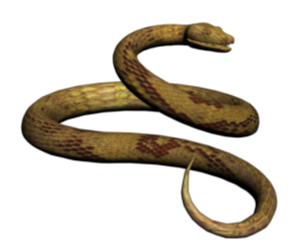
\includegraphics[scale=0.7]{Imagens/cobra01.png}
 \caption{Modelo da Cobra.}
\label{img:cobra}
\end{figure}


As animações para este personagem são:
\begin{itemize}
\item Rastejar;
\item Enrolar para o ataque;
\item Bote/Ataque;
\end{itemize}
\end{itemize}

\subsubsection{Urso}
O urso é o maior inimigo de Medrash e está presente somente na primeira
 fase do jogo. Se Medrash se aproximar muito dele, o urso se defenderá,
 perseguindo Medrash. Ao alcança-lo, o urso o ataca. O distanciamento de
 Medrash faz o urso esquecê-lo, voltando a patrulhar a região do mapa.
\begin{itemize}
\item {\bf Descrição física}
O urso pesa aproximadamente 400 Kg, tendo até 4 m de altura quando em
 posição bípede. Ele é muito robusto e apresenta pelagem marrom.


\begin{table}[H]
\begin{center}
\begin{tabular}{|c|c|}
\hline 
\textbf{Característica} & \textbf{Valor} \\ 
\hline 
Raio de detecção do personagem principal & 2K \\ 
\hline 
Raio de perda detecção do personagem principal & 6K \\ 
\hline 
Valor energético para o personagem principal & +90 p.p. \\ 
\hline 
Número de golpes para morrer & 9 \\ 
\hline 
Forma de ataque & Mordida \\ 
\hline 
Tipo de dano & Contusão \\ 
\hline 
Valor do dano & -15 p.p. \\ 
\hline 
\end{tabular} 
\caption{Características do Urso}
\end{center}
\end{table}


\item {\bf Concepção Artística}
O modelo definido para o urso está mostrado na Figura \ref{img:urso}.

\begin{figure}[H]
 \centering
 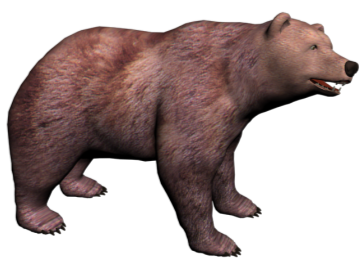
\includegraphics[scale=0.8]{Imagens/urso01.png}
 \caption{Modelo do urso}
\label{img:urso}
\end{figure}

As animações que o urso deverá ter são:
\begin{itemize}
\item Andar;
\item Correr;
\item Ficar sobre as patas traseiras;
\item Abraçar e morder Medrash.
\end{itemize}
\end{itemize}

\subsubsection{Jacaré}
O jacaré é um inimigo natural também encontrado na primeira fase do jogo.
 Vive ao redor de um rio, o qual Medrash é obrigado a atravessar para ir de
 um cenário à outro. O jacaré basicamente fica parado à margem do rio, e/ou
 nadando nele. Da mesma forma que a cobra, o jacaré só ataca se Medrash
 chegar muito próximo dele, nesse caso ele começa a persegui-lo tanto
 dentro como fora d'água. Se Medrash estiver muito perto do jacaré, este
 irá atacá-lo, ou seja, irá abocanhar Medrash. Caso Medrash se distancie o
 jacaré volta à sua posição inicial.
\begin{itemize}
\item {\bf Descrição Física}
O jacaré também possui aparência realista, com cerca de 2m de comprimento e
 pesando 80 Kg. Possui dentes afiados e maior agilidade dentro da água.
 Fora dela se torna muito mais lento, porém possui o mesmo poder de ataque.
 A tabela \ref{table:jacare} descreve as principais características do jacaré.

\begin{table}[H]
\begin{center}
\begin{tabular}{|c|c|}
\hline 
\textbf{Característica} & \textbf{Valor} \\ 
\hline 
Raio de detecção do personagem principal & 0,5K \\ 
\hline 
Raio de perda detecção do personagem principal & 6K \\ 
\hline 
Valor energético para o personagem principal & +60 p.p. \\ 
\hline 
Número de golpes para morrer & 6 \\ 
\hline 
Forma de ataque & Mordida \\ 
\hline 
Tipo de dano & Cortante/Contusão \\ 
\hline 
Valor do dano & -10 p.p. \\ 
\hline 
\end{tabular} 
\caption{Características do jacaré}
\label{table:jacare}
\end{center}
\end{table}

\item {\bf Concepção Artística}
Ainda não foi definido um modelo específico que representará o jacaré,
 porém, o modelo da Figura \ref{img:jacare} servirá como base para concepção do
 personagem.
\newpage
\begin{figure}[H]
 \centering
 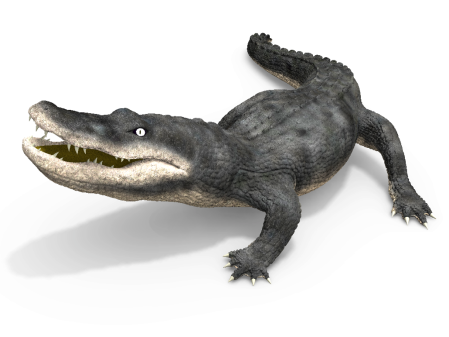
\includegraphics[scale=1]{Imagens/jacare01.png}
 \caption{Modelo do jacaré. (fonte: Htp://www.blendswap.com/blends/animals/alligator)}
\label{img:jacare}
\end{figure}

Animações que o jacaré deverá ter:
\begin{itemize}
\item Andar;
\item Nadar;
\item Abocanhar/Morder;
\end{itemize}
\end{itemize}
\subsubsection{Lobo}
O Lobo está presente na segunda fase do jogo, enquanto este está cortando caminho pelas montanhas para chegar à tribo Akanul. O Lobo foge de Medrash sempre que este está com a tocha acesa. Quando ela apaga, ele o persegue por todo o cenário até que Medrash acenda a tocha novamente
\begin{itemize}
\item {\bf Descrição Física}
O Lobo apresenta uma altura de aproximadamente 75 centímetros, se medido a partir do ombro, pesando cerca de 30 Kg.
\begin{table}[H]
\begin{center}
\begin{tabular}{|c|c|}
\hline 
\textbf{Característica} & \textbf{Valor} \\ 
\hline 
Raio de detecção do personagem principal & 0,5K \\ 
\hline 
Raio de perda detecção do personagem principal & 6K \\ 
\hline 
Valor energético para o personagem principal & +30 p.p. \\ 
\hline 
Número de golpes para morrer & 3 \\ 
\hline 
Forma de ataque & Mordida \\ 
\hline 
Tipo de dano & Cortante \\ 
\hline 
Valor do dano & -10 p.p. \\ 
\hline 
\end{tabular} 
\end{center}
\caption{Características do lobo}
\label{table:lobo}
\end{table}
\end{itemize}
\begin{itemize}
\newpage
\item {\bf Concepçao artística}

\begin{figure}[H]
 \centering
 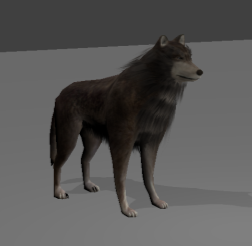
\includegraphics[scale=1]{Imagens/lobo01.png}
 \caption{Modelo do Lobo. (fonte: Htp://www.blendswap.com/blends/animals/wolf-for-bge-projekt/}
\label{img:lobo}
\end{figure}


As animações que o lobo deverá ter:
\begin{itemize}
\item {Andar;}
\item {Correr;}
\item {Uivar;}
\item {Morder;}

\end{itemize}

\end{itemize}
\subsubsection{Enxame de abelhas}
Presente na primeira fase do jogo, na área do Urso, o enxame de abelhas vive tranquilamente, até Medrash se aproximar demais. As abelhas não são fortes, mas se Medrash não fugir rapidamente elas podem ser um problema.
\begin{itemize}
\item {\bf Descrição física}
A colméia das abelhas é de aproximadamente 40 cm, com uma aparência simples. As colméias apresentam cerca de 400 a 500 abelhas.

As abelhas são pequenas, com aproximadamente 1 cm. 
\begin{table}[H]
\begin{center}
\begin{tabular}{|c|c|}
\hline 
\textbf{Característica} & \textbf{Valor} \\ 
\hline 
Raio de detecção do personagem principal & 0,25K \\ 
\hline 
Raio de perda detecção do personagem principal & 3K \\ 
\hline 
Valor energético para o personagem principal & Não convém\\ 
\hline 
Número de golpes para morrer & Não convém \\ 
\hline 
Forma de ataque & Picada \\ 
\hline 
Tipo de dano & Contusão \\ 
\hline 
Valor do dano & -1 p.p. \\ 
\hline 
\end{tabular} 
\end{center}
\caption{Características das abelhas}
\label{table:abelhas}
\end{table}
\end{itemize}
\begin{itemize}

\item {\bf Concepção artística}
O modelo de colméia será baseado nas imagens abaixo.

 \begin{figure}[H]
 \centering
 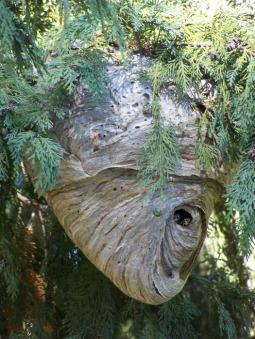
\includegraphics[scale=0.7]{Imagens/enxame01.png}
 \caption{Enxame de abelhas real. (Fonte: Htp://beesandwaspss.com/wasp-hive/)}
\label{img:abelhas}
\end{figure}
\end{itemize}
\newpage
\subsection{Tigre}
É o "chefe" da primeira fase, portanto o maior desafio para Medrash nesta etapa. Possui maior poder de ataque e é mais difícil de ser abatido.


O Tigre impede que Medrash avance para próxima tribo (segunda fase), portanto, o jogador só poderá prosseguir caso derrote o Tigre. Medrash poderá usar a lança ou o porrete para derrotá-lo, sendo que com a lança os ataques são mais eficientes. O tigre possui um ataque mais poderoso, tirando mais pontos de vida de Medrash. O tigre desfere ataques em forma de mordida e saltando sobre Medrash.
\begin{itemize}
\item {\bf Descrição física}
O tigre possui tamanho e aparência de um tigre real, com cerca de 1,2 m de altura e 3 m de comprimento (incluindo a cauda), pesando 300 Kg.

A tabela \ref{table:tigre} traz as principais características do tigre.
\end{itemize}
\begin{table}[H]
\begin{center}
\begin{tabular}{|c|c|}
\hline 
\textbf{Característica} & \textbf{Valor} \\ 
\hline 
Raio de detecção do personagem principal & Não convém \\ 
\hline 
Raio de perda detecção do personagem principal & Não convém \\ 
\hline 
Valor energético para o personagem principal & Não convém \\ 
\hline 
Número de golpes para morrer & 10 com a lança e 30 com o porrete \\ 
\hline 
Forma de ataque & Mordida/Patada\\ 
\hline 
Tipo de dano &  Contusão/Cortante \\ 
\hline 
Valor do dano & -15 p.p. \\ 
\hline 
\end{tabular} 
\end{center}
\caption{Características Tigre}
\label{table:tigre}
\end{table}
\begin{itemize}
\item {\bf Concepção artística}

A figura \ref{img:tigre} demonstra o modelo do tigre.
\newpage
\begin{figure}[H]
 \centering
 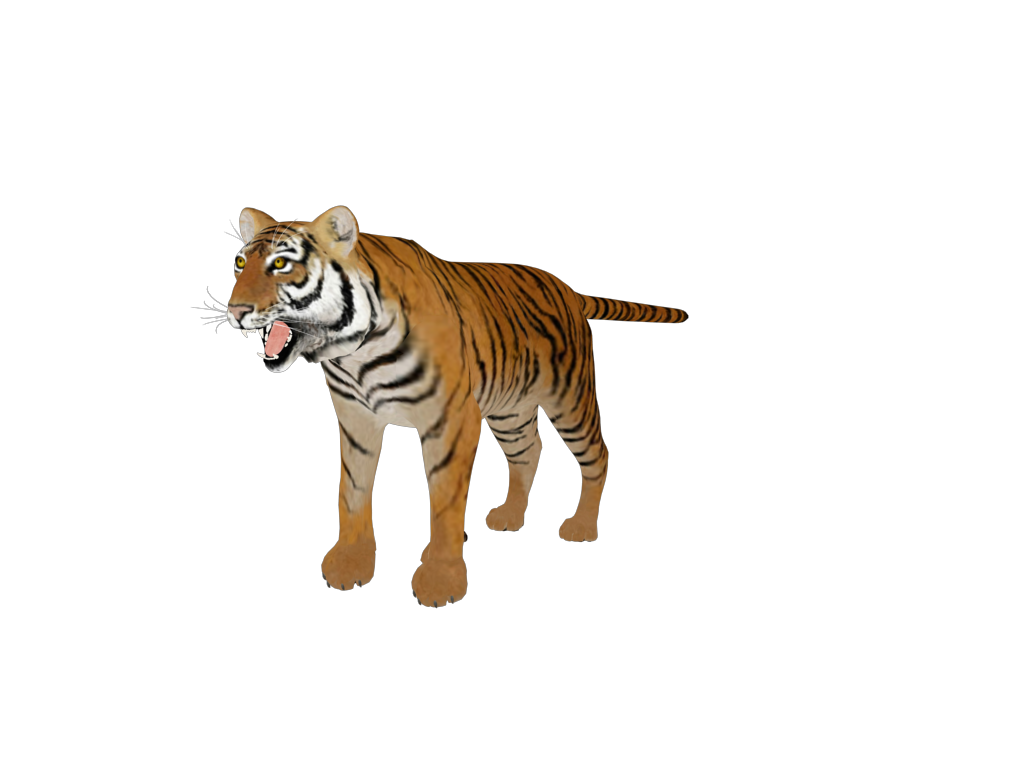
\includegraphics[scale=0.3]{Imagens/tigre01.png}
 \caption{Modelo do Tigre}
\label{img:tigre}
\end{figure}

As animações do tigre são:
\begin{itemize}
\item {Andar;}
\item {Correr;}
\item {Posição para o ataque;}
\item {Ataque com salto;}
\item {Morder;}
\end{itemize}
\end{itemize}

\subsubsection{Balazar}
Balasar é o arqui-inimigo de Medrash. É o líder da tribo Luskan e tem como determinação destruir todas as outras tribos do mundo para se tornar líder absoluto de tudo. Balasar sequestra Sora e escraviza todos os outros.
\begin{itemize}
\item {\bf Descrição física}
Balazar é um personagem gordo, 1.65m de altura com 150 Kg.
\end{itemize}
\newpage
\begin{table}[H]
\begin{center}
\begin{tabular}{|c|c|}
\hline 
\textbf{Característica} & \textbf{Valor} \\ 
\hline 
Raio de detecção do personagem principal & Não convém \\ 
\hline 
Raio de perda detecção do personagem principal & Não convém \\ 
\hline 
Valor energético para o personagem principal & Não convém \\ 
\hline 
Número de golpes para morrer & 15 com machado\\ 
\hline 
Forma de ataque & Ataque com porrete\\ 
\hline 
Tipo de dano &  Contusão/Cortante \\ 
\hline 
Valor do dano & -10 p.p. \\ 
\hline 
\end{tabular} 
\end{center}
\caption{Características de Balazar}
\label{table:balazar}
\end{table}
\begin{itemize}
\item{\bf Concepção artística} O modelo que representará Balazar é apresentado abaixo.
 \begin{figure}[H]
 \centering
 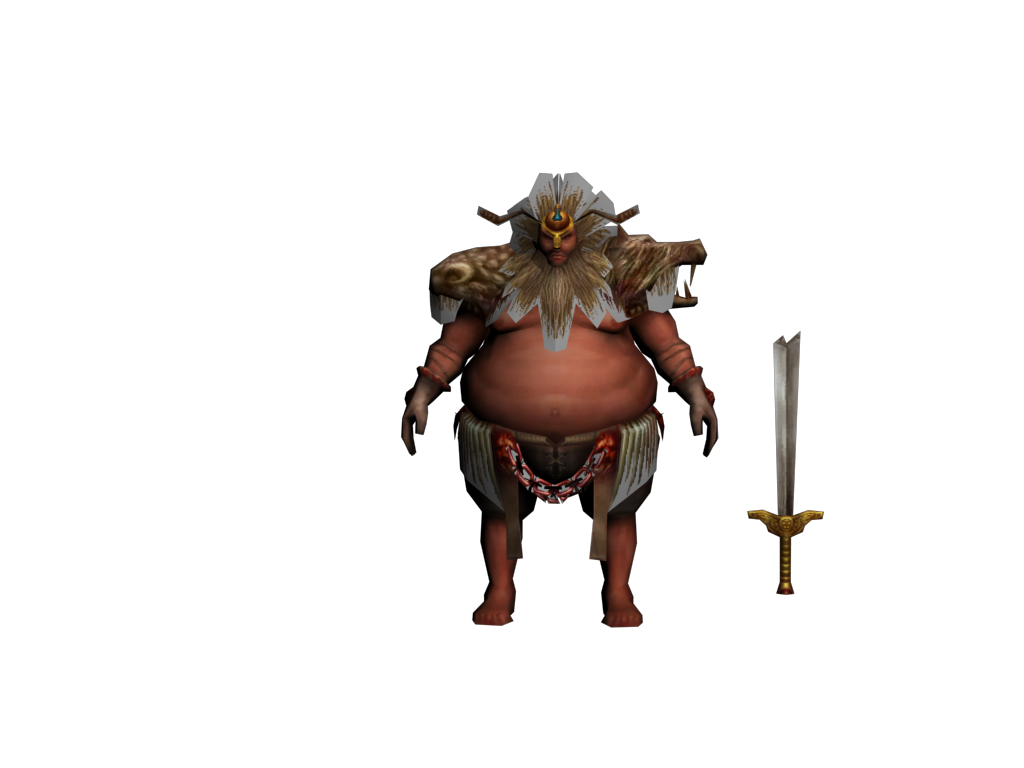
\includegraphics[scale=0.33]{Imagens/inimigo01.png}
 \caption{Modelo do Balazar. (Fonte: : Htp://www.3dmodelfree.com/models/26570-0.Hm)}
\label{img:balazar}
\end{figure}

Balazar deverá ter as seguintes animações: 
\begin{itemize}
\item {Atacar;}
\item {Atordoado;}
\item {Correr;}
\item {Cair;}
\end{itemize}
\end{itemize}
\subsubsection{Guerreiros inimigos da tribo Luskan}
Representam os humanos inimigos de Medrash. Dentre todos os inimigos da tribo Luskan, esses guerreiros são os mais fracos. Os guerreiros de Luskan aparecem no jogo a partir da parte dois da segunda fase, durante um ataque da tribo a tribo Mara-Kai. Nesse ataque participarão dois tipos de guerreiros da tribo Luskan, um que irá atear fogo na morada defendida por Medrash, e outro que encontrará em combate direto com nosso herói.

\begin{itemize}
\item{\bf Descrição física}
Esses guerreiros são os mais fracos da tribo Luskan. Com aproximadamente 1, 70m e pesando cerca de 70kg, possuem fisionomia muito parecida com a de Medrash. Seus ataques são baseados basicamente em luta corporal, mas podem também portar pequenas armas, porém, nada que se compare aos guerreiros mais fortes da tribo Luskan.
\end{itemize}

A tabela \ref{table:luskans} descreve as características básicas desses guerreiros.
\begin{table}[H]
\begin{center}
\begin{tabular}{|c|c|}
\hline 
\textbf{Característica} & \textbf{Valor} \\ 
\hline 
Número de golpes para morrer & 3\\ 
\hline 
Forma de ataque & Corporal\\ 
\hline 
Tipo de dano &  Contusão \\ 
\hline 
Valor do dano & -10 p.p. \\ 
\hline 
\end{tabular} 
\end{center}
\caption{Características dos guerreiros luskans}
\label{table:luskans}
\end{table}
\begin{itemize}
\item{\bf Concepção artística}
O modelo que representará os guerreiros de Luskan é basicamente um humano com adaptações de vestimenta e armamento para se adaptar ao período do jogo.

Possivelmente será utilizado o mesmo modelo para essa classe de guerreiros, com algumas diferenciações apenas na forma física e/ou maneira de se vestir.

As figuras abaixo servirão de inspiração para a concepção do modelos de guerreiro.
\newpage
 \begin{figure}[H]
 \centering
 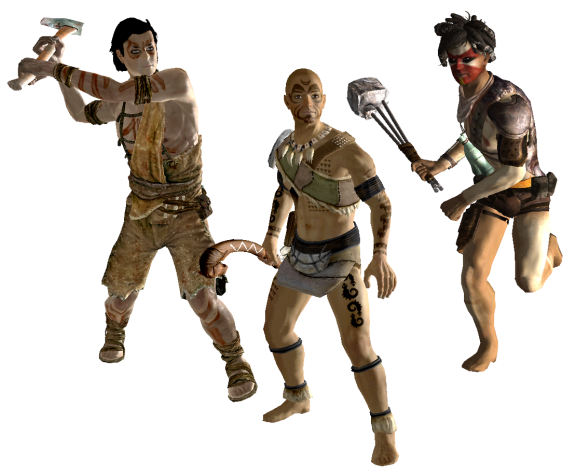
\includegraphics[scale=0.5]{Imagens/guerreiro01.png}
 \caption{- Guerreiros tribais do jogo Fallout3 (fonte: Htp://fallout.wikia.com/wiki/File:Tribal.png)}
\label{img:guerreiro01}
 \centering
 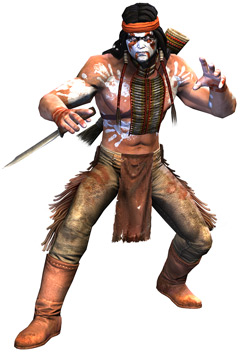
\includegraphics[scale=0.5]{Imagens/guerreiro02.png}
 \caption{Guerreiro Apache (fonte Htp://xboxlivemedia.ign.com/
 xboxlive/image/article/
 109/1094953/deadliest-warrior-the-game-20100604025247714.jpg)}
\end{figure}
\end{itemize}

\subsubsection{Escravos}
Os escravos representam os habitantes das tribos Ari e Mara-kai que foram capturados pelos guerreiros da tribo Luskan. Os escravos estarão presentes na terceira fase do jogo, onde ficarão presos por estacas flamejantes. Serão divididos em três grupos. Nessa etapa Medrash deverá derrotar os inimigos da tribo Luskan para poder libertar os respectivos escravos. Tendo derrotado todos os guerreiros inimigos, Medrash poderá destruir as estacas que guardam os escravos, terminando, todos os escravos estarão livres.

\begin{itemize}
\item{\bf Descrição física}
Os escravos são humanos com a mesma aparência dos demais habitantes de sua tribo. Porém, devido ao aprisionamento, encontram-se visivelmente mais magros e debilitados.
\end{itemize}
\begin{itemize}
\item{\bf Concepção artística}
Como mencionado, os escravos serão modelos normais de humanos. Possivelmente sendo variações do modelo que representará os guerreiros inimigos, ou Medrash.


As imagens abaixo serão utilizadas como referência para a criação dos modelos.

\begin{figure}[H]
 \centering
 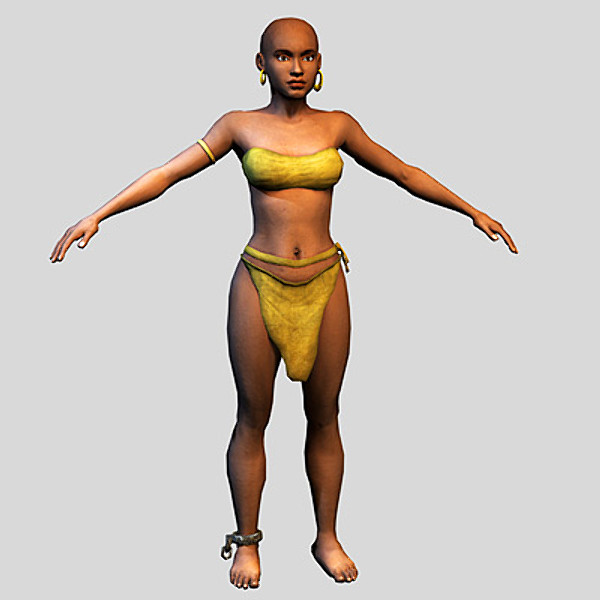
\includegraphics[scale=0.5]{Imagens/mulher01.png}
 \caption{Modelo de escrava (fonte: Htp://www.turbosquid.com/3d-models/3d-female-slave-model/506597)}
\label{img:mulher}
\end{figure}
\newpage
\begin{figure}[H]
 \centering
 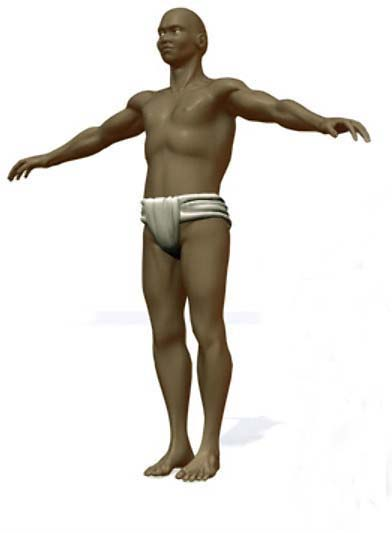
\includegraphics[scale=0.5]{Imagens/escravo01.png}
 \caption{Modelo de escravo (fonte: Htp://www.turbosquid.com/3d-models/3ds-slave/334940 )}
\label{img:escrava}
\end{figure}
\end{itemize}
\subsubsection{Porrete 2}
O porrete é a arma principal de Balazar. Esta arma apresenta um grande poder de destruição contra Medrash.

Abaixo é apresentada a arma de Balazar.

\begin{figure}[H]
 \centering
 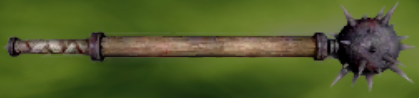
\includegraphics[scale=1]{Imagens/porrete02.png}
 \caption{Modelo de Porrete para Balazar (Fonte: Jogo Infinity blade)}
\label{img:porrete02}
\end{figure}